%%%%%%%%%%%%%%%%%%%%%%%%%%%%%%%%%%%%%%%%%
% University/School Laboratory Report
% LaTeX Template
% Version 3.1 (25/3/14)
%
% This template has been downloaded from:
% http://www.LaTeXTemplates.com
%
% Original author:
% Linux and Unix Users Group at Virginia Tech Wiki 
% (https://vtluug.org/wiki/Example_LaTeX_chem_lab_report)
%
% License:
% CC BY-NC-SA 3.0 (http://creativecommons.org/licenses/by-nc-sa/3.0/)
%
% Modified by:
% Bartlomiej Dybisz
% Warsaw university of Technology
%
%%%%%%%%%%%%%%%%%%%%%%%%%%%%%%%%%%%%%%%%%

%----------------------------------------------------------------------------------------
%	PACKAGES AND DOCUMENT CONFIGURATIONS
%----------------------------------------------------------------------------------------

\documentclass{article}

\usepackage[version=3]{mhchem} % Package for chemical equation typesetting
\usepackage{siunitx} % Provides the \SI{}{} and \si{} command for typesetting SI units
\usepackage{graphicx} % Required for the inclusion of images
\usepackage{amsmath} % Required for some math elements 
\usepackage{url} % for bibliograpy links
\usepackage{float} % To force image to stand still
\usepackage[export]{adjustbox}
\usepackage[usenames, dvipsnames]{color} % to color some important remarks
\usepackage{caption}
\usepackage{wrapfig}
\usepackage{subcaption}
\urlstyle{same}  % (for bibliography links
\setlength\parindent{0pt} % Removes all indentation from paragraphs
%\usepackage{array}

\newenvironment{conditions}
  {\par\vspace{\abovedisplayskip}\noindent\begin{tabular}{>{$}l<{$} @{${}\equiv{}$} l}}
  {\end{tabular}\par\vspace{\belowdisplayskip}}
  
 \usepackage{amsfonts} 
\renewcommand{\labelenumi}{\alph{enumi}.} % Make numbering in the enumerate environment by letter rather than number (e.g. section 6)

%\usepackage{times} % Uncomment to use the Times New Roman font

%----------------------------------------------------------------------------------------
%	DOCUMENT INFORMATION
%----------------------------------------------------------------------------------------

\title{Analysis and Processing of Biometric Images \\ Laboratory 3} % Title

\author{Bartłomiej \textsc{Dybisz}} % Author name

\date{\today} % Date for the report

\begin{document}

\maketitle % Insert the title, author and date

\begin{center}
\begin{tabular}{l r}
Date Performed: & October 31 , 2015 \\ % Date the experiment was performed
Instructor: & mgr Piotr Panasiuk % Instructor/supervisor
\end{tabular}
\end{center}

% If you wish to include an abstract, uncomment the lines below
% \begin{abstract}
% Abstract text
% \end{abstract}

%----------------------------------------------------------------------------------------
%	SECTION 1
%----------------------------------------------------------------------------------------

\section{Objectives}

% If you have more than one objective, uncomment the below:
\begin{description}
\item[Convolution Filters] \hfill \\
\item[High Pass Filter] \hfill \\
\item[Low Pass Filter] \hfill \\
\item[Gaussian Filter] \hfill \\
\item[Sobel Filter] \hfill \\
\item[Dilation] \hfill \\
\item[Erosion] \hfill \\
\item[Flood Fill Algorithm] \hfill \\
\item[Region Extraction] \hfill \\
\end{description}

\subsection{Definitions}
\label{definitions}
\textcolor{red}{Remark:} throughout this report I will assume that each of red, green, blue channels of a pixel can take values from $0$ to $1$. It is imposed by JavaFX 8 - technology used to implement algorithms.

\begin{description}
\item[Convolution]
A convolution is an integral that expresses the amount of overlap of one function g as it is shifted over another function f. It therefore "blends" one function with another  \cite{convolution_wolphram}. 

In other words, convolution gives the area overlap between the two functions as a function of the amount that one of the original functions is translated \cite{convolution_wiki}.

Formally, for functions $f(x)$ and $g(x)$ of a continuous variable x, convolution is defined as:
\begin{equation} \label{conv_one_var_cont}
f(x) * g(x) = \int_{-\infty}^{\infty} f(\tau) \cdot g(x - \tau) d\tau
\end{equation}
, where $*$ means convolution operation, $\cdot$ represents common multiplication and $\tau$ is a "shifting variable".

Equation \ref{conv_one_var_cont} can be easily transformed to discrete form as follows:
\begin{equation} \label{conv_one_var_disc}
f[x] * g[x] = \sum_{k=-\infty}^{\infty} f[k] \cdot g[x-k]
\end{equation}
This form will be of particular interest for us, since it can be (more or less) directly applied to an image as showed in the next subsection.

\item[Convolution Filters]
As mentioned, one can ad hoc transform equation \ref{conv_one_var_disc} into two variable case:
\begin{equation} \label{two_var_conv_one_var_disc}
f[x,y] * g[x,y] =\sum_{n_{1}=-\infty}^{\infty} \sum_{n_{2}=-\infty}^{\infty} f[n_{1}, n_{2}] \cdot g[x-n_{1}, y - n_{2}]
\end{equation}
, but for our purposes (as explained in a moment) we will use a slightly modified version of equation \ref{two_var_conv_one_var_disc}, namely:
\begin{equation} \label{final_two_var_conv_one_var_disc}
f[x,y] * g[x,y] =\sum_{n_{1}=k_{1}}^{k_{2}} \sum_{n_{2}=k_{3}}^{k_{4}} f[n_{1}, n_{2}] \cdot g[x+n_{1}, y + n_{2}]
\end{equation}
,where:
\begin{conditions} 
  n_{1}, n_{2} \in \mathbb{N}& auxiliary shifting variables\\
  k_{1}, k_{2}, k_{3}, k_{4} \in \mathbb{N}& size restriction to convolution matrix (kernel)\\
 (x,y) \in \mathbb{N}^{2}     &  pixel of interest's position on an image in XY coordinates \\   
 f[x,y] : \mathbb{N}^{2} \rightarrow \mathbb{N} &  convolution matrix (kernel) \\
 g[x,y] : \mathbb{N}^{2} \rightarrow \mathbb{N} & an image as a matrix of pixels values
\end{conditions}

Equation \ref{two_var_conv_one_var_disc} has been changed due to obsolete $g[x-k]$ notation of equation \ref{conv_one_var_disc}. In this way we can omit left-right flipping when calculating consecutive pixels.

In addition, we restrict $g[x,y]$ by $k$'s variables, because we want our convolution matrix to be finite. 
In this case we can think of $f[x,y]$ as a frame, which we move over some pixel $(x,y)$ of an image $g[x,y]$. Then by applying equation \ref{final_two_var_conv_one_var_disc} we sum all values of $g$ over
$ \langle x + k_1; x+ k_2 \rangle \cup \langle y + k_3 ; y + k_4 \rangle$ interval multiplied by appropriate values of $f$. 

As an example let us assume that:
\begin{conditions} 
  g[x,y] : \langle 1; 5 \rangle \cup \langle 1 ; 7 \rangle \rightarrow \mathbb{N} & some very small image\\
  f[x,y] : \langle -1; 1 \rangle \cup \langle -1 ; 1 \rangle \rightarrow \mathbb{N} & kernel matrix
\end{conditions}

In such a case we can present both of them in form of matrices of some natural values. Let us assume that figure \ref{fig:example_repr} defines $f[x,y]$ and $g[x,y]$ in terms of matrices.
\begin{figure}[H]
\centering
\begin{subfigure}{.4\textwidth}
  \centering
  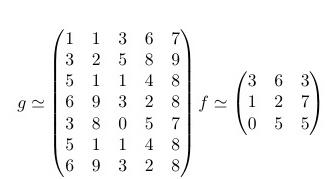
\includegraphics[width=0.95\linewidth]{_Figures/example_11.jpg}
  \caption{}
  \label{fig:example_repr}
\end{subfigure}%
\begin{subfigure}{.4\textwidth}
  \centering
  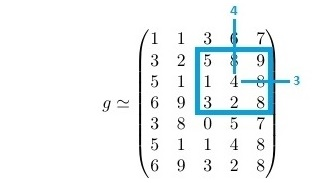
\includegraphics[width=0.95\linewidth]{_Figures/example_12.jpg}
  \caption{}
  \label{fig:example_43}
\end{subfigure}%
\caption{}
\label{fig:results_tresh}
\end{figure}

Now we want to apply convolution for let us say pixel $(4,3)$. Figure \ref{fig:example_43} represents region of interest. Equation \ref{final_two_var_conv_one_var_disc} for this case takes following form:
\begin{equation} 
\begin{split}
f[4,3] * g[4,3] =\sum_{n_{1}=-1}^{1} \sum_{n_{2}=-1}^{1} f[n_{1}, n_{2}] \cdot g[4+n_{1}, 3 + n_{2}] \\
= f[-1, -1] \cdot g[3, 2] + f[-1, 0] \cdot g[3, 3] + f[-1, 1] \cdot g[3, 4] \\
+ f[0, -1] \cdot g[3, 2] + f[0, 0] \cdot g[3, 3] + f[0, 1] \cdot g[0, 4] \\
+ f[1, -1] \cdot g[3, 2] + f[1, 0] \cdot g[3, 3] + f[1, 1] \cdot g[0, 4] \\
= 3 * 5 + 1 * 1 + 0 * 3 \\
+ 6 * 8 + 2 * 4 + 5 * 2 \\
+ 3 * 9 + 7 * 8 + 8 * 5 \\
= 205
\end{split}
\end{equation}

In this way pixel of output image, positioned at $(4,3)$ will have value $205$. When we apply convolution to all pixels in $g$ we will get an output (filtered) image.

\begin{figure}
\noindent
\begin{minipage}{0.3\textwidth}% adapt widths of minipages to your needs
	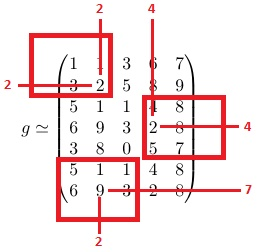
\includegraphics[width=\linewidth]{_Figures/conv_filter_border.jpg} 
	\caption{}
	\label{fig:caution}
\end{minipage}%
\hfill%
\begin{minipage}{0.6\textwidth}\raggedleft
\textcolor{red}{Caution:} Border cases i.e. cases when there is no corresponding $g[x,y]$ value for some value of $f[x,y]$ (see figure \ref{fig:caution} for reference), will be treated as special ones. In such a case pixel of interest will keep its value from $g$ function.
\end{minipage}
\end{figure}

For the rest of the paper we will use only $3 \times 3$ kernel matrices, hence $k_1 = k_3 = -1$ and $k_2 = k_4 = 1$.

\item[High Pass Filter]
\item[Low Pass Filter]
\item[Gaussian Filter]
\item[Sobel Filter]
\item[Dilation]
\item[Erosion]
\item[Flood Fill Algorithm]
\end{description} 

 
%----------------------------------------------------------------------------------------
%	SECTION 2
%----------------------------------------------------------------------------------------

\section{Experimental Data}


%----------------------------------------------------------------------------------------
%	SECTION 3
%----------------------------------------------------------------------------------------

\newpage
\section{Sample Code}
This section contains code snippets with algorithms implementation. Each figures is provided with appropriate description either in caption or in method's comment. 

%
% CLASS DIAGRAM
%
\subsection{Operations Class Diagram}




%----------------------------------------------------------------------------------------
%	SECTION 4
%----------------------------------------------------------------------------------------

\section{Results and Conclusions}


%----------------------------------------------------------------------------------------
%	BIBLIOGRAPHY
%----------------------------------------------------------------------------------------
\newpage

\begin{thebibliography}{1}
	\bibitem{convolution_wolphram} \url{http://mathworld.wolfram.com/Convolution.html}
	\bibitem{convolution_wiki} \url{https://en.wikipedia.org/wiki/Convolution#Discrete_convolution}
	\bibitem{convolution_equations} \url{https://graphics.stanford.edu/courses/cs178/applets/convolution.html}
\end{thebibliography}

%----------------------------------------------------------------------------------------


\end{document}